% Page 042 — page imprimée 38
% Contenu seul : le préambule, l'en-tête et la pagination sont gérés par meyrueis.tex

nombreux et les premiers touristes circulaient beaucoup par ce moyen. Il introduisit également
le cinéma à Meyrueis vers 1910 en transformant l’écurie de la maison Cabanel en salle
obscure. Il avait acheté à Nîmes un piano qui était tenu par la fille du célèbre guide de Martel :
Hippolyte Caussé dit Poulard, et lors des séances on descendait les fauteuils de la maison pour
installer les notables et les clients de l’Hôtel de France venus découvrir la grotte de Dargilan.
Mobilisé en 1914, il devint un véritable mécanicien pendant la guerre. De retour au pays en 1919,
il intensifia la vente des machines agricoles amorcée depuis le début du siècle et se lança dans
la vente des automobiles. Ses premiers véhicules étaient des De Dion et Bouton pour le compte
du garage Champayrac d’Alès. Paul Malafosse était le seul mécanicien à trente kilomètres à la
ronde et avait des clients sur les Causses, mais aussi jusqu’à Nant, Florac ou Valleraugue. En 1920
il acheta une torpédo De Dion et Bouton et se lança dans le taxi (courses régulières à Millau et
Sauclières en correspondance avec les trains, hospitalisations à Millau et bien sûr excursions
touristiques : mont Aigoual, Dargilan, gorges du Tarn). Parallèlement il créait avec son ami
Liausson de Saint-Jean-du-Bruel la « société saint-jeantaise de transport » pour exploiter les
lignes d’autobus Millau-Florac, Millau-Meyrueis et Millau-Saint-Jean-du-Bruel et Sauclières
(1920). En 1921, il prend un premier contact avec la maison Citroën portant sur la vente de deux
modèles B2 (acquis par les instituteurs de Sainte-Enimie et de Fraissinet-de-Fourques). Dès lors la
construction d’un véritable garage s’impose car la circulation automobile devenait importante
surtout en été. Ce fut chose faite avec la construction en 1925-1926 du Grand Garage Malafosse,
« agent exclusif Citroën et mandataire des huiles et carburants Esso » qu’il dirige épaulé par sa
fille unique qui assure la comptabilité et le taxi !, et son gendre Léon Giraud. Nous avons choisi
de développer l’exemple de ce vrai Lozérien (natif du Mas-Saint-Chély sur le causse Méjean), car
il a su trouver les voies d’une réussite individuelle et familiale en saisissant les opportunités
qu’ouvrait le développement de l’automobile stimulé puissamment dans le sud du département
par la croissance de l’activité touristique. Le Garage Malafosse de Meyrueis (devenu Giraud par la
suite), « plus petite concession Citroën de France », exclusivité assurant jusqu’à aujourd’hui sa
réputation en Lozère, servit de base arrière en 1928 et 1929 pour la préparation de La croisière
jaune d’André Citroën. Les autocanelles C4 s’entraînaient sur le causse Méjean qui dit-on
ressemblerait au désert de Gobi et étaient entretenues ou modifiées au Grand Garage de Meyrueis.
Notons que le plateau du Méjean apparaissait toujours comme un site extrême pouvant être
comparé à de difficiles contrées lointaines. Désert de Gobi dans les années vingt, il avait été en
1879 comparé à « un petit Pamir » par Alphonse Lequeutre. Le développement de l’automobile
est certes encore réservé à une minorité plus ou moins fortunée, mais il entraînera en se
démocratisant deux changements de fond pour le tourisme : une pratique beaucoup plus
individuelle des séjours touristiques qui seront moins liés aux voyages de groupe et aux séjours
organisés et une découverte beaucoup plus éclairée des sites à visiter, les véhicules parvenant
finalement à pénétrer partout les itinéraires variés que se choisissent les conducteurs (voir à ce
propos les suggestions de Paul Cabouat : \textit{En automobile dans les Cévennes dans Causses et Cévennes},
1928). L’automobile permet de réaliser des itinéraires spécifiques au gré de chacun. Conseillé par
Charles Bost et piloté par un jeune neveu, le pasteur Charles Dhombre descend en 1926 du
mont Lozère et fait des zigzags d’automobile sur les routes de crête des Cévennes huguenotes
nous livrant le récit de son périple dans un petit livre improvisé mais si bien vu : \textit{Si
j’étais en pays camisard}. Il cherche à connaître les hauts lieux de la résistance protestante,
sur la trace des assemblées et des combats, et à comprendre l’âme de ce pays différente de
celle des terres catholiques situées plus au nord. Avec l’automobile, il pratique en éclaireur
une forme de tourisme religieux (qui tient presque du pèlerinage) et culturel qui s’amplifiera
dans la seconde moitié du XXe siècle.

\begin{center}
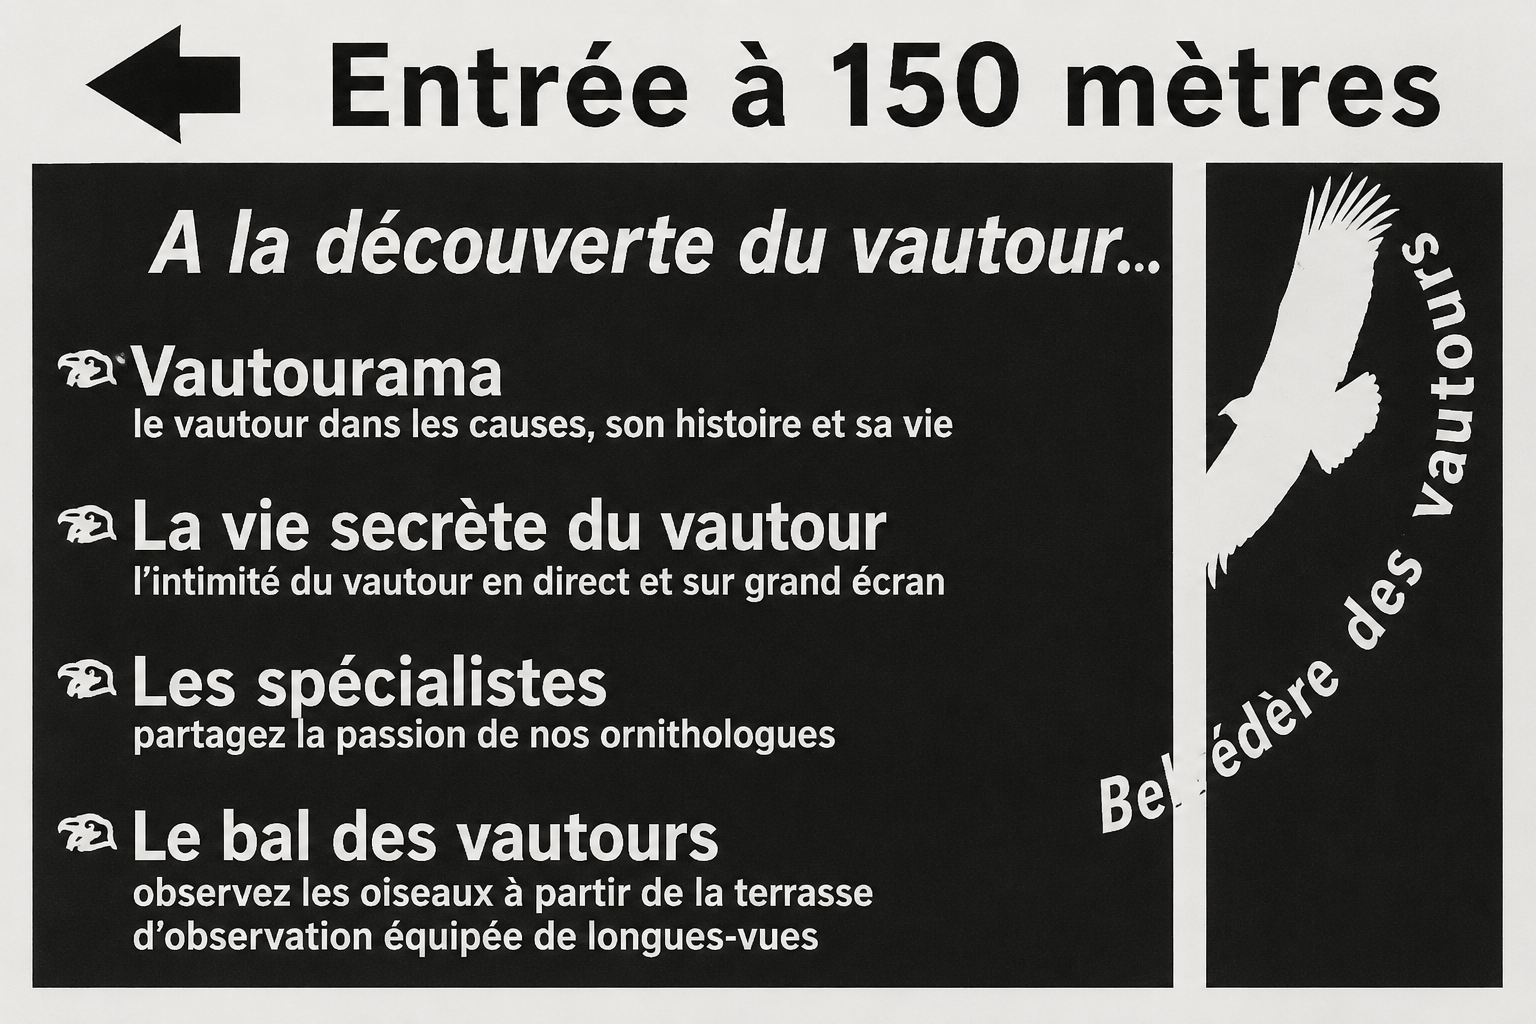
\includegraphics[width=0.82\textwidth]{imgs/042.png}
\end{center}
